\chapter{Invertible Transforms and Optimization} \label{app:ch6:invertible}
To see this, let us consider the work from \cite{rippel_spectral_2015} where
filters are parameterized in the Fourier domain. 

If we define the DFT as the orthonormal version, i.e.\ let:
$$ U_{ab} = \frac{1}{\sqrt{N}} \exp\{ \frac{-2j\pi ab}{N} \} $$
%
then call $X = \DFT{x}$. In matrix form the 2-D DFT is then:

\begin{eqnarray}
  X &=& \DFT{x} = UxU \\
  x &=& \IFT{X} = U^*YU^* 
\end{eqnarray}

When it comes to gradients, these become:
\begin{eqnarray}
  \dydx{L}{X} &=& U \dydx{L}{x} U = \DFT{\dydx{L}{x}} \label{eq:ch6:dft_grad}\\
  \dydx{L}{x} &=& U^* \dydx{L}{X} U^* = \IFT{\dydx{L}{X}}
\end{eqnarray}

Now consider a single filter parameterized in the DFT and spatial domains
presented with the exact same data and with the same \ltwo\ regularization
$\epsilon$ and learning rate $\eta$. Let
the spatial filter at time $t$ be $\vec{w}_t$, the Fourier-parameterized
filter be $\hat{\vec{w}}_t$, and let 

\begin{equation}
  \hat{\vec{w}}_1 = \F{DFT}\{\vec{w}_1\} \label{eq:ch6:initial_condition}
\end{equation}
%
After presenting both systems with the same minibatch of samples $\mathcal{D}$
and calculating the gradient $\dydx{L}{\vec{w}}$ we update both parameters:

\begin{eqnarray}
  \vec{w}_2 & = & \vec{w}_1 - \eta \left(
    \dydx{L}{\vec{w}} + \epsilon \vec{w}_1 \right) \\
    &=& (1-\eta\epsilon)\vec{w}_1 - \eta \dydx{L}{\vec{w}} \\
  \hat{\vec{w}}_2 & = & \hat{\vec{w}}_1 - \eta \left(
     \dydx{L}{\hat{\vec{w}}} + \epsilon \hat{\vec{w}}_1 \right)  \\
     &=& (1-\eta\epsilon)\hat{\vec{w}_1} - \eta \dydx{L}{\hat{\vec{w}}} \\
\end{eqnarray}

Where we have shortened the gradient of the loss evaluated at the current
parameter values to $\delta_{\vec{w}}$ and $\delta_{\hat{\vec{w}}}$.
We can then compare the effect the new parameters would have on the next
minibatch by calculating $\F{DFT}^{-1} \{\hat{\vec{w}}_2 \}$. Using
equations~\ref{eq:ch6:dft_grad} and ~\ref{eq:ch6:initial_condition} we then get:

\begin{eqnarray}
  \IFT{\hat{\vec{w}}_2} &=& \IFT{(1-\eta\epsilon)\hat{\vec{w}_1} - \eta\ \dydx{L}{\hat{\vec{w}}}} \\       
                        & = & (1-\eta\epsilon)\vec{w}_1 - \eta\ \IFT{ \dydx{L}{\hat{\vec{w}}}} \\
                        & = & (1-\eta\epsilon)\vec{w}_1 - \eta \dydx{L}{\vec{w}} \\
                        & = & \vec{w}_2
\end{eqnarray}

\subsection{Regularization}
If we use $\ell_1$ then the above doesn't hold.

\subsection{Optimization}
If we us adam things r different.

This does not hold for the Adam \cite{kingma_adam:_2014} or Adagrad \cite{}
optimizers, which automatically rescale the learning rates for each parameter
based on estimates of the parameter's variance. Rippel et.\ al.\ use this fact
in their paper \cite{rippel_spectral_2015}.

\chapter{$\DTCWT$ Single Subband Gains}\label{app:ch6:dtcwt}

\begin{figure}
  \centering
  \begin{tikzpicture}
    \matrix (m1) [minimum height=4mm, column sep=6mm, align=center]
	{
	%--------------------------------------------------------------------
		\node[coordinate]                  (m00) {};    &
		\node[coordinate]                  (m01) {};          &
		\node[dspsquare]                   (m02) {$A(z)$};          &
		\node[circle,draw,inner sep=1pt]   (m03) {\downsamplertext{M}}; &
		\node[dspnodeopen,dsp/label=above] (m04) {$X_a(z)$};          &
		\node[circle,draw,inner sep=1pt]   (m07) {\upsamplertext{M}}; &
		\node[dspsquare]                   (m08) {$C(z)$};          &
		\node[coordinate]                  (m09) {};          &
		\node[coordinate]                  (m0X) {};          \\
		%--------------------------------------------------------------------
		\node[dspnodefull]                 (m10) {};          &
		\node[coordinate]                  (m11) {};          &
		\node[coordinate]                  (m12) {};    &
		\node[coordinate]                  (m13) {};          &
		\node[coordinate]                  (m14) {};    &
		\node[coordinate]                  (m17) {};          &
		\node[coordinate]                  (m18) {};    &
		\node[dspadder]                    (m19) {};          &
		\node[]     (m1X) {};          \\
		%--------------------------------------------------------------------
		\node[coordinate]                  (m20) {};    &
		\node[coordinate]                  (m21) {};          &
		\node[dspsquare]                   (m22) {$B(z)$};          &
		\node[circle,draw,inner sep=1pt]   (m23) {\downsamplertext{M}}; &
		\node[dspnodeopen,dsp/label=below] (m24) {$X_b(z)$};          &
		\node[circle,draw,inner sep=1pt]   (m27) {\upsamplertext{M}}; &
		\node[dspsquare]                   (m28) {$D(z)$};          &
		\node[coordinate]                  (m29) {};          &
		\node[coordinate]                  (m2X) {};          \\
		%--------------------------------------------------------------------
	};
	\draw[dspline] (m10) -- (m11);
	\draw[dspline] (m11) -- (m01);
	\draw[dspline] (m11) -- (m21);
	\foreach \i in {0,2} {
    	\draw[dspconn] (m\i1) -- (m\i2);
    	\draw[dspconn] (m\i2) -- (m\i3);
    	\draw[dspline] (m\i3) -- (m\i4);
    	\draw[dspconn] (m\i4) -- (m\i7);
    	\draw[dspconn] (m\i7) -- (m\i8);
    	\draw[dspline] (m\i8) -- (m\i9);
	}
  \node[left=0pt of m10] (left) {$X(z)$};
  \node[below=9pt of m24] (bottom) {};
  \draw[dspconn] (m09) -- node[right, yshift=5pt] {$Y_a(z)$} (m19);
  \draw[dspconn] (m29) -- node[right, yshift=-5pt] {$Y_b(z)$} (m19);
  \draw[dspconn] (m19) -- node[right, xshift=5pt] {$Y(z)$} (m1X);
	
\end{tikzpicture}

  \mycaption{Block Diagram of 1-D $\DTCWT$}{Note the top and bottom paths are
  through the wavelet or scaling functions from just level m ($M=2^m$). Figure
  based on Figure~4 in \cite{kingsbury_complex_2001}.}
  \label{fig:ch6:dtcwt_two_tree}
\end{figure}

Let us consider one subband of the $\DTCWT$. This includes the coefficients from
both tree A and tree B. For simplicity in this analysis we will consider the 1-D
$\DTCWT$ without the channel parameter $c$. If we only keep coefficients from a given
subband and set all the others to zero, then we have a reduced tree as shown in
\autoref{fig:ch6:dtcwt_two_tree}. The end to end transfer function is:
%
\begin{equation}
  \frac{Y(z)}{X(z)} = \frac{1}{M} \sum_{k=0}^{M-1} \left[A(W^k z)C(z) + B(W^k z)D(z)\right]
  \label{eq:ch6:aliasing}
\end{equation}
%
where the aliasing terms are formed from the addition of the rotated z
transforms, i.e.\ when $k \neq 0$.

\begin{theorem} \label{thm:ch6:shiftinv}
  Suppose we have complex filters $P(z)$ and $Q(z)$ with support only in the
  positive half of the frequency space. If $A(z) = 2\real{P(z)}$, $B(z) =
  2\imag{P(z)}$, $C(z) = 2\real{Q(z)}$ and $D(z) = -2\imag{Q(z)}$, then the aliasing
  terms in \eqref{eq:ch6:aliasing} are nearly zero and the system is nearly
  shift invariant.
\end{theorem}

\begin{proof}
  See section 4 of \cite{kingsbury_complex_2001} for the full proof of
  this, and section 7 for the bounds on what `nearly' shift invariant means. 
  In short, from the definition of $A, B, C$ and $D$ it follows that:  
  \begin{eqnarray*}
    A(z) &=& P(z) + P^*(z) \\
    B(z) &=& -j(P(z) - P^*(z)) \\
    C(z) &=& Q(z) + Q^*(z) \\
    D(z) &=& j(Q(z) - Q^*(z))
  \end{eqnarray*}
  where $H^*(z) = \sum_n h^*[n]z^{-n}$ is the $Z$-transform of the complex
  conjugate of the complex filter $h$. This reflects the purely positive
  frequency support of $P(z)$ to a purely negative one. Substituting these into
  \eqref{eq:ch6:aliasing} gives:
  \begin{equation}
    A(W^k z)C(z) + B(W^k z)D(z) = 2P(W^kz)Q(z) + 2P^*(W^kz)Q^*(z)
    \label{eq:ch6:complex_filts}
  \end{equation}
 Using \eqref{eq:ch6:complex_filts}, Kingsbury shows that it is easier to design
 single side band filters so $P(W^kz)$ does not overlap with $Q(z)$ and
 $P^*(W^kz)$ does not overlap with $Q^*(z)$ for $k \neq 0$.
\end{proof}

Using \autoref{thm:ch6:shiftinv} \eqref{eq:ch6:aliasing} reduces to:
\begin{equation}
 \frac{Y(z)}{X(z)} = \frac{1}{M}\left[ A(z)C(z) + B(z)D(z) \right]
  \label{eq:ch6:aliasing_cancel}
\end{equation}

Let us extend this idea to allow for any linear gain applied to the passbands
(not just zeros and ones). Ultimately, we may want to allow for nonlinear
operations applied to the wavelet coefficients, but we initially restrict
ourselves to linear gains so that we can build from a sensible base. In
particular, if we want to have gains applied to the wavelet coefficients, it
would be nice to maintain the shift invariant properties of the $\DTCWT$.

\begin{figure}
  \centering
  \begin{tikzpicture}
    \matrix (m1) [row sep=5mm, column sep=6mm,align=center,anchor=center]
	{
	%--------------------------------------------------------------------
		\node[coordinate]                  (m00) {};    &
		\node[coordinate]                  (m01) {};          &
		\node[dspsquare]                   (m02) {$A(z)$};          &
		\node[circle,draw,inner sep=1pt]   (m03) {\downsamplertext{M}}; &
		\node[dspnodeopen,dsp/label=above] (m04) {$U_a(z)$};          &
    \node[rectangle,draw,inner sep=2pt](m05) {$G_{aa}(z)$}; &
		\node[dspnodeopen,dsp/label=above] (m06) {$V_a(z)$};          &
		\node[circle,draw,inner sep=1pt]   (m07) {\upsamplertext{M}}; &
		\node[dspsquare]                   (m08) {$C(z)$};          &
		\node[coordinate]                  (m09) {};          &
		\node[coordinate]                  (m0X) {};          \\
		%--------------------------------------------------------------------
      \node[dspnodefull]                 (m10) {};          &
		\node[coordinate]                  (m11) {};          &
		\node[coordinate]                  (m12) {};    &
		\node[coordinate]                  (m13) {};          &
		\node[coordinate]                  (m14) {};    &
		\node[coordinate]                  (m15) {};          &
		\node[coordinate]                  (m16) {};    &
		\node[coordinate]                  (m17) {};          &
		\node[coordinate]                  (m18) {};    &
		\node[dspadder]                    (m19) {};          &
    \node[]                            (m1X) {$Y(z)$};          \\
		%--------------------------------------------------------------------
		\node[coordinate]                  (m20) {};    &
		\node[coordinate]                  (m21) {};          &
		\node[dspsquare]                   (m22) {$B(z)$};          &
		\node[circle,draw,inner sep=1pt]   (m23) {\downsamplertext{M}}; &
		\node[dspnodeopen,dsp/label=below] (m24) {$U_b(z)$};          &
      \node[rectangle,draw,inner sep=2pt](m25) {$G_{bb}(z)$}; &
		\node[dspnodeopen,dsp/label=below] (m26) {$V_b(z)$};          &
		\node[circle,draw,inner sep=1pt]   (m27) {\upsamplertext{M}}; &
		\node[dspsquare]                   (m28) {$D(z)$};          &
		\node[coordinate]                  (m29) {};          &
		\node[coordinate]                  (m2X) {};          \\
		%--------------------------------------------------------------------
  };
	\draw[dspline] (m10) -- (m11);
	\draw[dspline] (m11) -- (m01);
	\draw[dspline] (m11) -- (m21);
	\foreach \i in {0,2} {
    	\draw[dspconn] (m\i1) -- (m\i2);
    	\draw[dspconn] (m\i2) -- (m\i3);
    	\draw[dspline] (m\i3) -- (m\i4);
    	\draw[dspconn] (m\i4) -- (m\i5);
    	\draw[dspline] (m\i5) -- (m\i6);
    	\draw[dspconn] (m\i6) -- (m\i7);
    	\draw[dspconn] (m\i7) -- (m\i8);
    	\draw[dspline] (m\i8) -- (m\i9);
	}
	%\draw[dspflow] (m04) --  (m06);
	%\draw[dspflow] (m24) -- (m26);
  \draw[dspconn] (m24) -- node[draw,pos=0.7,inner sep=2pt,fill=white] {$G_{ba}(z)$} (m06);
  \draw[dspconn] (m04) -- node[draw,pos=0.7,inner sep=2pt,fill=white] {$G_{ab}(z)$} (m26);
  \draw[dspconn] (m09) -- node[right] {$Y_a(z)$} (m19);
  \draw[dspconn] (m29) -- node[right] {$Y_b(z)$} (m19);
	\draw[dspconn] (m19) -- (m1X);
  \node[left=0pt of m10] (left) {$X(z)$};
  \node[below=10pt of m24] (bottom) {};
	
\end{tikzpicture}

  \mycaption{Block Diagram of 1-D $\DTCWT$}{Note the top and bottom paths are
  through the wavelet or scaling functions from just level m ($M=2^m$). Figure
  based on Figure~4 in \cite{kingsbury_complex_2001}.}
  \label{fig:ch6:dtcwt_two_tree_gain}
\end{figure}

\autoref{fig:ch6:dtcwt_two_tree_gain} shows a block diagram of the extension of 
the above to general gains. This is a two port network with four individual
transfer functions. Let the transfer fucntion from $U_i$ to $V_j$
be $G_{ij}$ for $i, j \in \{a, b\}$. Then $V_a$ and $V_b$ are:
\begin{eqnarray}
  V_a(z) &=& U_a(z)G_{aa}(z) + U_b(z)G_{ba}(z) \\
         &=& \frac{1}{M} \sum_k X(W^{k} z^{1/k}) \left[A(W^k z^{1/k})G_{aa}(z) +
             B(W^k z^{1/k}) G_{ba}(z) \right] \\
  V_b(z) &=& U_a(z)G_{ab}(z) + U_b(z)G_{bb}(z) \\
         &=& \frac{1}{M} \sum_k X(W^{k} z^{1/k}) \left[A(W^k z^{1/k})G_{ab}(z) +
             B(W^k z^{1/k}) G_{bb}(z) \right] 
\end{eqnarray}
%
Further, $Y_a$ and $Y_b$ are:
\begin{eqnarray}
  Y_a(z) &=& C(z)V_a(z^M) \\
  Y_b(z) &=& D(z)V_b(z^M)
\end{eqnarray}
%
Then the end to end transfer function is:
\begin{equation}
  \begin{split}
  % \begin{multline}
    Y(z) = Y_{a}(z) + Y_{b}(z) = \frac{1}{M} \sum_{k=0}^{M-1} X(W^k z)
    & \left[  A(W^kz)C(z)G_{aa}(z^k) + B(W^kz)D(z)G_{bb}(z) + \right. \\
    & \left. \hphantom{[}  B(W^kz)C(z)G_{ba}(z^k) + A(W^kz)D(z)G_{ba}(z) \right] 
    \label{eq:ch6:transfer}
  % \end{multline}
  \end{split}
\end{equation}

\begin{theorem}\label{thm:ch6:shiftinvgain}
  If we let $G_{aa}(z^k) = G_{bb}(z^k) = G_r(z^k)$ and $G_{ab}(z^k) = -G_{ba}(z^k) = G_i(z^k)$
  then the end to end transfer function is shift invariant.
\end{theorem}
\begin{proof}
  Using the above substitutions, the terms in the square brackets of
  \eqref{eq:ch6:transfer} become:
  \begin{equation}\label{eq:ch6:realimag}
    G_r(z^k)\left[A(W^kz)C(z) + B(W^kz)D(z)\right] + G_i(z^k)\left[A(W^kz)D(z) - B(W^kz)C(z)\right]
  \end{equation}
  \autoref{thm:ch6:shiftinv} already showed that the $G_r$ terms are shift
  invariant and reduce to $A(z)C(z) + B(z)D(z)$. To prove the same for the $G_i$
  terms, we follow the same procedure. Using our definitions of $A, B, C, D$
  from \autoref{thm:ch6:shiftinv} we note that:
  %
  \begin{eqnarray}
    A(W^kz)D(z) - B(W^kz)C(z) &=& j\left[P(W^kz) + P^*(W^kz)\right]\left[Q(z) -Q^*(z)\right] +\\
                              &&j\left[P(W^kz) -P^*(W^kz)\right]\left[Q(z) + Q^*(z)\right] \\
                              &=& 2j\left[P(W^kz)Q(z) - P^*(W^kz)Q^*(z)\right]
  \end{eqnarray}
  We note that the difference
  between the $G_r$ and $G_i$ terms is just in the sign of the negative
  frequency parts, $AD - BC$ is the Hilbert pair of $AC+BD$. To prove shift
  invariance for the $G_r$ terms in \autoref{thm:ch6:shiftinv}, we ensured that
  $P(W^kz)Q(z) \approx 0$ and $P^*(W^kz)Q^*(z) \approx 0$ for $k\neq 0$. We can
  use this again here to prove the shift invariance of the $G_i$ terms in
  \eqref{eq:ch6:realimag}. This completes our proof.
\end{proof}

Using \autoref{thm:ch6:shiftinvgain}, the end to end transfer function with the
gains is now
\begin{eqnarray}
  \frac{Y(z)}{X(z)} &=& \frac{2}{M} \left[G_r(z^{M}) \left(A(z)C(z) + B(z)D(z)\right)
  + G_i(z^{M}) \left(A(z)D(z) - B(z)C(z)\right) \right] \\
  &=& \frac{2}{M}\left[G_r(z^{M}) \left(PQ + P^*Q^*\right)
  + jG_i(z^{M}) \left(PQ - P^*Q^*\right) \right]  \label{eq:ch6:end2end}
\end{eqnarray}

Now we know can assume that our $\DTCWT$ is well designed and extracts frequency
bands at local areas, then our complex filter $G(z)=G_r(z) + jG_i(z)$ allows us
to modify these passbands (e.g.\ by simply scaling if $G(z) = C$, or by more
complex functions.


\subsection{Backpropagation Analysis}
We start with the commonly known property that for a convolutional block, the
gradient with respect to the input is the gradient with respect to the output
convolved with the time reverse of the filter. More formally, if 
$Y(z) = H(z) X(z)$:
%
\begin{equation}\label{eq:ch6:backprop}
  \Delta X(z) = H(z^{-1}) \Delta Y(z)
\end{equation}
%
where $H(z^{-1})$ is the $Z$-transform of the time/space reverse of $H(z)$,
$\Delta Y(z) \triangleq \dydx{L}{Y}(z)$ is the gradient of the loss with respect
to the output, and $\Delta X(z) \triangleq \dydx{L}{X}(z)$ is the gradient of
the loss with respect to the input. If H were complex, the first term in
\autoref{eq:ch6:backprop} would be $\bar{H}(1/\bar{z})$, but as each individual
block in the $\DTCWT$ is purely real, we can use the simpler form. 

Assume we already have access to the quantity $\Delta Y(z)$ (this is the input
to the backwards pass). \autoref{fig:ch6:bwd_pass} illustrates the
backpropagation procedure. An interesting result is that the backwards pass of
an inverse wavelet transform is equivalent to doing a forward wavelet
transform.\footnote{As shown in \autoref{fig:ch6:bwd_pass}, the analysis and
synthesis filters have to be swapped and time reversed. For orthogonal wavelet
transforms, the synthesis filters are already the time reverse of the analysis
filters, so no change has to be done. The q-shift filters of the $\DTCWT$
\cite{kingsbury_design_2003} have this property.} Similarly, the backwards pass
of the forward transform is equivalent to doing the inverse transform. The
weight update gradients are then calculated by finding 
\textbf{FIX this - make it not use the $\DTCWT$ to get delta v}.
$\Delta V(z) = \DTCWT\left\{ \Delta Y(z) \right\}$ and then convolving with the 
time reverse of the saved wavelet coefficients from the forward pass - $U(z)$.

\begin{gather}
  \Delta G_r(z) = \Delta V_r(z) U_r(z^{-1}) + \Delta V_i(z) U_i(z^{-1})  \label{eq:ch6:gr_update}\\
  \Delta G_i(z) =  -\Delta V_r(z) U_i(z^{-1}) + \Delta V_i(z) U_r(z^{-1})  \label{eq:ch6:gi_update} 
\end{gather}

Unsurprisingly, the passthrough gradients have similar form to
\autoref{eq:ch6:end2end}:
\begin{equation}\label{eq:ch6:passthrough}
    \Delta X(z) = \frac{2\Delta Y(z)}{M} \left[G_r(z^{-M})\left( PQ + P^*Q^* \right)\right. + 
      \left. jG_i(z^{-M}) \left(PQ-P^*Q^* \right) \right] 
\end{equation}
where we have dropped the $z$ terms on $P(z), Q(z), P^*(z), Q^*(z)$ for brevity.

Note that we only need to evaluate equations
~\ref{eq:ch6:gr_update},\ref{eq:ch6:gi_update},\ref{eq:ch6:passthrough} over the
support of $G(z)$ i.e., if it is a single number we only need to calculate
$\left.\Delta G(z)\right\rvert_{z=0}$.

\begin{figure}[ht]
  \centering
  % \subfloat[]{%
    % 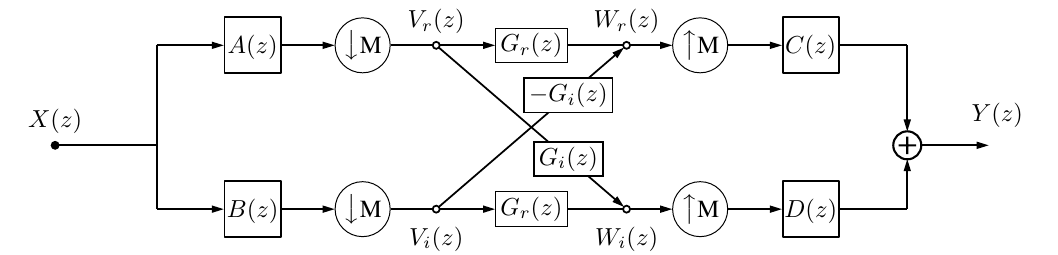
\includegraphics[width=.85\textwidth]{freqlearn/images/top_block.png}
    % \label{fig:ch6:fwd_pass}
  % }
   % \newline
  % \subfloat[]{%
    % 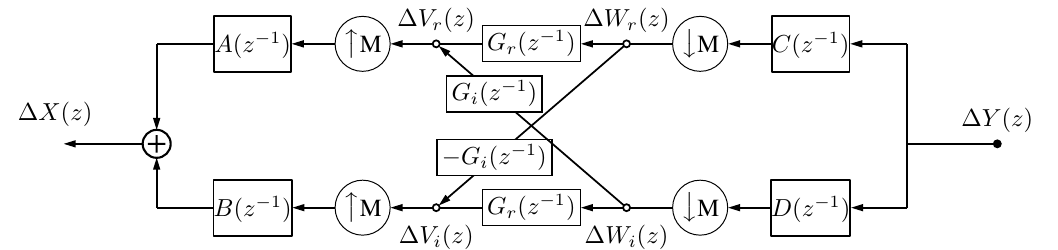
\includegraphics[width=.85\textwidth]{freqlearn/images/bottom_block.png}
    % \label{fig:ch6:bwd_pass}
  % }
  \makebox[\textwidth][c]{%
    \resizebox{1.1\textwidth}{!}{\begin{tikzpicture}
    \matrix (m1) [row sep=5mm, column sep=6mm,align=center,anchor=center]
	{
	% %--------------------------------------------------------------------
		% \node[coordinate]                  (m00) {};    &
		% \node[coordinate]                  (m01) {};          &
		% \node[dspsquare]                   (m02) {$A(z)$};          &
		% \node[circle,draw,inner sep=1pt]   (m03) {\downsamplertext{M}}; &
		% \node[dspnodeopen,dsp/label=above] (m04) {$V_r(z)$};          &
		% \node[rectangle,draw,inner sep=2pt](m05) {$G_r(z)$}; &
		% \node[dspnodeopen,dsp/label=above] (m06) {$W_r(z)$};          &
		% \node[circle,draw,inner sep=1pt]   (m07) {\upsamplertext{M}}; &
		% \node[dspsquare]                   (m08) {$C(z)$};          &
		% \node[coordinate]                  (m09) {};          &
		% \node[coordinate]                  (m0X) {};          \\
		% %--------------------------------------------------------------------
		% \node[]                            (m10) {$X(z)$};          &
		% \node[coordinate]                  (m11) {};          &
		% \node[coordinate]                  (m12) {};    &
		% \node[coordinate]                  (m13) {};          &
		% \node[coordinate]                  (m14) {};    &
		% \node[coordinate]                  (m15) {};          &
		% \node[coordinate]                  (m16) {};    &
		% \node[coordinate]                  (m17) {};          &
		% \node[coordinate]                  (m18) {};    &
		% \node[dspadder]                    (m19) {};          &
    % \node[]                            (m1X) {$Y(z)$};          \\
		% %--------------------------------------------------------------------
		% \node[coordinate]                  (m20) {};    &
		% \node[coordinate]                  (m21) {};          &
		% \node[dspsquare]                   (m22) {$B(z)$};          &
		% \node[circle,draw,inner sep=1pt]   (m23) {\downsamplertext{M}}; &
		% \node[dspnodeopen,dsp/label=below] (m24) {$V_i(z)$};          &
		% \node[rectangle,draw,inner sep=2pt](m25) {$G_r(z)$}; &
		% \node[dspnodeopen,dsp/label=below] (m26) {$W_i(z)$};          &
		% \node[circle,draw,inner sep=1pt]   (m27) {\upsamplertext{M}}; &
		% \node[dspsquare]                   (m28) {$D(z)$};          &
		% \node[coordinate]                  (m29) {};          &
		% \node[coordinate]                  (m2X) {};          \\
		% %--------------------------------------------------------------------
		% &&&&&&&&& \\
		\node[coordinate]                  (m00a) {};    &
		\node[coordinate]                  (m01a) {};          &
		\node[dspsquare]                   (m02a) {$A\left(z^{-1}\right)$};          &
		\node[circle,draw,inner sep=1pt]   (m03a) {\upsamplertext{M}}; &
		\node[dspnodeopen,dsp/label=above] (m04a) {$\Delta U_r(z)$};          &
		%\node[coordinate]                  (m05) {}; &
		\node[rectangle,draw,inner sep=2pt](m05a) {$G_r\left(z^{-1}\right)$}; &
		\node[dspnodeopen,dsp/label=above] (m06a) {$\Delta V_r(z)$};          &
		\node[circle,draw,inner sep=1pt]   (m07a) {\downsamplertext{M}}; &
		\node[dspsquare]                   (m08a) {$C\left(z^{-1}\right)$};          &
		\node[coordinate]                  (m09a) {};          &
		\node[coordinate]                  (m0Xa) {};          \\
		%--------------------------------------------------------------------
		%\node[coordinate]  (m10) {$\Delta X(z)$};          &
    \node[]                            (m10a) {$\Delta X(z)$}; &
		\node[dspadder]                    (m11a) {};          &
		\node[coordinate]                  (m12a) {};    &
		\node[coordinate]                  (m13a) {};          &
		\node[coordinate]                  (m14a) {};    &
		\node[coordinate]                  (m15a) {};          &
		\node[coordinate]                  (m16a) {};    &
		\node[coordinate]                  (m17a) {};          &
		\node[coordinate]                  (m18a) {};    &
		\node[coordinate]                  (m19a) {};          &
		\node[]                            (m1Xa) {$\Delta Y(z)$};          \\
		%--------------------------------------------------------------------
		\node[coordinate]                  (m20a) {};    &
		\node[coordinate]                  (m21a) {};          &
		\node[dspsquare]                   (m22a) {$B\left(z^{-1}\right)$};          &
		\node[circle,draw,inner sep=1pt]   (m23a) {\upsamplertext{M}}; &
		\node[dspnodeopen,dsp/label=below] (m24a) {$\Delta U_i(z)$};          &
		%\node[coordinate]                  (m25) {}; &
		\node[rectangle,draw,inner sep=2pt](m25a) {$G_r\left(z^{-1}\right)$}; &
		\node[dspnodeopen,dsp/label=below] (m26a) {$\Delta V_i(z)$};          &
		\node[circle,draw,inner sep=1pt]   (m27a) {\downsamplertext{M}}; &
		\node[dspsquare]                   (m28a) {$D\left(z^{-1}\right)$};          &
		\node[coordinate]                  (m29a) {};          &
		\node[coordinate]                  (m2Xa) {};          \\
		%--------------------------------------------------------------------
	};
	% \draw[dspline] (m10) -- (m11);
	% \draw[dspline] (m11) -- (m01);
	% \draw[dspline] (m11) -- (m21);
	% \foreach \i in {0,2} {
      % \draw[dspconn] (m\i1) -- (m\i2);
      % \draw[dspconn] (m\i2) -- (m\i3);
      % \draw[dspline] (m\i3) -- (m\i4);
      % \draw[dspconn] (m\i4) -- (m\i5);
      % \draw[dspline] (m\i5) -- (m\i6);
      % \draw[dspconn] (m\i6) -- (m\i7);
      % \draw[dspconn] (m\i7) -- (m\i8);
      % \draw[dspline] (m\i8) -- (m\i9);
	% }
	% %\draw[dspflow] (m04) --  (m06);
	% %\draw[dspflow] (m24) -- (m26);
	% \draw[dspconn] (m24) -- node[draw,pos=0.7,inner sep=2pt,fill=white] {$-G_i(z)$} (m06);
	% \draw[dspconn] (m04) -- node[draw,pos=0.7,inner sep=2pt,fill=white] {$G_i(z)$} (m26);
	% \draw[dspconn] (m09) -- (m19);
	% \draw[dspconn] (m29) -- (m19);
	% \draw[dspconn] (m19) -- (m1X);
	\draw[dspconn] (m11a) -- (m10a);
	\draw[dspconn] (m01a) -- (m11a);
	\draw[dspconn] (m21a) -- (m11a);
	\foreach \i in {0,2} {
    	\draw[dspconn] (m\i9a) -- (m\i8a);
    	\draw[dspconn] (m\i8a) -- (m\i7a);
    	\draw[dspline] (m\i7a) -- (m\i6a);
    	\draw[dspconn] (m\i6a) -- (m\i5a);
    	\draw[dspline] (m\i5a) -- (m\i4a);
    	\draw[dspconn] (m\i4a) -- (m\i3a);
    	\draw[dspconn] (m\i3a) -- (m\i2a);
    	\draw[dspline] (m\i2a) -- (m\i1a);
	}
	%\draw[dspflow] (m04) --  (m06);
	%\draw[dspflow] (m24) -- (m26);
	\draw[dspconn] (m06a) -- node[draw,pos=0.7,inner sep=2pt,fill=white] {$-G_i\left(z^{-1}\right)$} (m24a);
	\draw[dspconn] (m26a) -- node[draw,pos=0.7,inner sep=2pt,fill=white] {$G_i\left(z^{-1}\right)$} (m04a);
	\draw[dspline] (m09a) -- (m19a);
	\draw[dspline] (m29a) -- (m19a);
	\draw[dspline] (m19a) -- (m1Xa);
	
\end{tikzpicture}
}
  }
  \mycaption{Forward and backward block diagrams for $\DTCWT$ gain layer}{Based
    on Figure~4 in \cite{kingsbury_complex_2001}. Ignoring the $G$ gains, the
    top and bottom paths (through $A, C$ and $B, D$ respectively) make up the
    the real and imaginary parts for \emph{one subband} of the dual tree system.
    Combined, $A+jB$ and $C-jD$ make the complex filters necessary to have
    support on one side of the Fourier domain (see
    \autoref{fig:ch6:dtcwt_bands}). Adding in the complex gain $G_r + jG_i$, we
    can now attenuate/shape the impulse response in each of the subbands. To
    allow for learning, we need backpropagation. The bottom diagram indicates
    how to pass gradients $\Delta Y(z)$ through the layer. Note that upsampling
    has become downsampling, and convolution has become convolution with the
  time reverse of the filter (represented by $z^{-1}$ terms).}
  \label{fig:ch6:fwd_bwd}
\end{figure}




